% -*- mode: LaTeX; TeX-PDF-mode: t; -*-
\input{./.econtexRoot}\documentclass[\econtexRoot/BufferStockTheory]{subfiles}
\input{./.econtexRoot}\input{\LaTeXInputs/econtex_onlyinsubfile}
\onlyinsubfile{\externaldocument{\LaTeXGenerated/BufferStockTheory}} % Get xrefs -- esp to appendix -- from main file; only works properly if main file has already been compiled;

%\renewcommand{\LtxDir}{}
\onlyinsubfile{\renewcommand{\LtxDir}{../LaTeX/}}


\begin{document}

\hypertarget{ApndxBalancedGrowthcNrmAndCov}{}
\section{Apparent Balanced Growth in \texorpdfstring{$\cNrmAvg$}{c} and \texorpdfstring{$\cov(\cNrm,\PermLvl)$}{cov(c,p)}}\label{sec:ApndxBalancedGrowthcNrmAndCov}

%\providecommand{\GroFac}{\Omega}\renewcommand{\GroFac}{\Omega}

Section~\ref{subsec:Covariances} demonstrates some propositions under the assumption that, when an economy satisfies the {\GICRaw}, there will be constant growth factors $\GroFac_{\cNrmAvg}$ and $\GroFac_{\cov}$ respectively for $\cNrmAvg$ (the average value of the consumption ratio) and $\cov(\cNrm,\PermLvl)$.  In the case of a Szeidl-invariant economy, the main text shows that these are $\GroFac_{\cNrmAvg}=1$ and $\GroFac_{\cov}=\PermGroFac$.  If the economy is Harmenberg- but not Szeidl-invariant, no proof is offered that these growth factors will be constant.

\subsection{\texorpdfstring{$\log \cNrm$}{log c} and \texorpdfstring{$\log \left(\cov(\cNrm,\PermLvl)\right)$}{log cov(c,p)} Grow Linearly}
Figures~\ref{fig:logcNrm} and~\ref{fig:logcov} plot the results of simulations of an economy that satisfies Harmenberg- but not Szeidl-invariance with a population of 4 million agents over the last 1000 periods (of a 2000 period simulation).\footnote{For an exposition of our implementation of Harmenberg's method, see \href{https://github.com/econ-ark/BufferStockTheory/blob/master/Appendices/ApndxHarKmenberg.pdf}{this supplemental appendix.}}  The first figure shows that $\log \cNrmAvg$ increases apparently linearly.  The second figure shows that $\log (-\cov(\cNrm,\PermLvl))$ also increases apparently linearly.  (These results are produced by the notebook \href{https://github.com/econ-ark/BufferStockTheory/blob/master/Code/Python/ApndxBalancedGrowthcNrmAndCov.ipynb}{\texttt{ApndxBalancedGrowthcNrmAndCov.ipynb}}).

\pagebreak
\begin{figure}[ht]
  \centerline{
    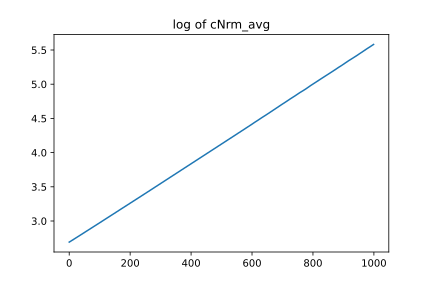
\includegraphics[width=4in]{\FigDir/logcNrm}
  }
  \caption{Appendix: $\log ~\mathfrak{c}$ Appears to Grow Linearly}\label{fig:logcNrm}
\end{figure}
\begin{figure}[ht]
  \centerline{
    \includegraphics[width=4in]{\FigDir/logcov}
  }
  \caption{Appendix: $\log ~(-\cov(\cNrm,\PermLvl))$ Appears to Grow Linearly}\label{fig:logcov}
\end{figure}


\end{document}
\endinput

% Local Variables:
% eval: (setq TeX-command-list  (assq-delete-all (car (assoc "BibTeX" TeX-command-list)) TeX-command-list))
% eval: (setq TeX-command-list  (assq-delete-all (car (assoc "BibTeX" TeX-command-list)) TeX-command-list))
% eval: (setq TeX-command-list  (assq-delete-all (car (assoc "BibTeX" TeX-command-list)) TeX-command-list))
% eval: (setq TeX-command-list  (assq-delete-all (car (assoc "BibTeX" TeX-command-list)) TeX-command-list))
% eval: (setq TeX-command-list  (assq-delete-all (car (assoc "Biber"  TeX-command-list)) TeX-command-list))
% eval: (add-to-list 'TeX-command-list '("BibTeX" "bibtex ../LaTeX/%s" TeX-run-BibTeX nil t                                                                              :help "Run BibTeX") t)
% eval: (add-to-list 'TeX-command-list '("BibTeX" "bibtex ../LaTeX/%s" TeX-run-BibTeX nil (plain-tex-mode latex-mode doctex-mode ams-tex-mode texinfo-mode context-mode) :help "Run BibTeX") t)
% TeX-PDF-mode: t
% TeX-file-line-error: t
% TeX-debug-warnings: t
% LaTeX-command-style: (("" "%(PDF)%(latex) %(file-line-error) %(extraopts) -output-directory=../LaTeX %S%(PDFout)"))
% TeX-source-correlate-mode: t
% TeX-parse-self: t
% eval: (cond ((string-equal system-type "darwin") (progn (setq TeX-view-program-list '(("Skim" "/Applications/Skim.app/Contents/SharedSupport/displayline -b %n ../LaTeX/%o %b"))))))
% eval: (cond ((string-equal system-type "gnu/linux") (progn (setq TeX-view-program-list '(("Evince" "evince --page-index=%(outpage) ../LaTeX/%o"))))))
% eval: (cond ((string-equal system-type "gnu/linux") (progn (setq TeX-view-program-selection '((output-pdf "Evince"))))))
% TeX-parse-all-errors: t
% End:
